\documentclass[a4paper, 12pt]{article}
\usepackage[total={17cm,25cm}, top=2.5cm, left=2.5cm, right=2.5cm,  includefoot]{geometry}
\usepackage[utf8]{inputenc}
\usepackage{array}
\usepackage{multirow}
\usepackage{hhline}
\usepackage{gensymb}
\usepackage{graphicx}
\graphicspath{ {} }
\usepackage[czech]{babel}
\usepackage{enumitem}
\usepackage{pdfpages}
\usepackage{amsmath}
\usepackage{verbatim}
\usepackage{listings}
\usepackage{hyperref}
\usepackage{amssymb}


\pagestyle{empty} % vypne číslování stránek




%\usepackage[OT2,OT1]{fontenc}
\newcommand\cyr
{
\renewcommand\rmdefault{wncyr}
\renewcommand\sfdefault{wncyss}
\renewcommand\encodingdefault{OT2}
\normalfont
\selectfont
}
\DeclareTextFontCommand{\textcyr}{\cyr}
\def\cprime{\char"7E }
\def\cdprime{\char"7F }
\def\eoborotnoye{\char’013}
\def\Eoborotnoye{\char’003}


\begin{document}



\begin{titlepage}
\begin{center}
\noindent
\Large \textbf{České vysoké učení technické v Praze }\\ Fakulta stavební
\vspace{5cm}

\huge

%vložení loga cvut
%\begin{figure}[h!]
%	\centering
%	\includegraphics[width=7cm]{logo.png}
%\end{figure}

\vspace{0.5cm}

155ADKG: Digitální model terénu \\

\vspace{10cm}




\Large
Michael Kala\\
Anna Zemánková \\

\end{center}

\end{titlepage}




\pagestyle{plain}     % zapne obyčejné číslování
\setcounter{page}{1}  % nastaví čítač stránek znovu od jedné

%\tableofcontents
%\newpage

\section{Zadání}

\begin{figure}[h!]
	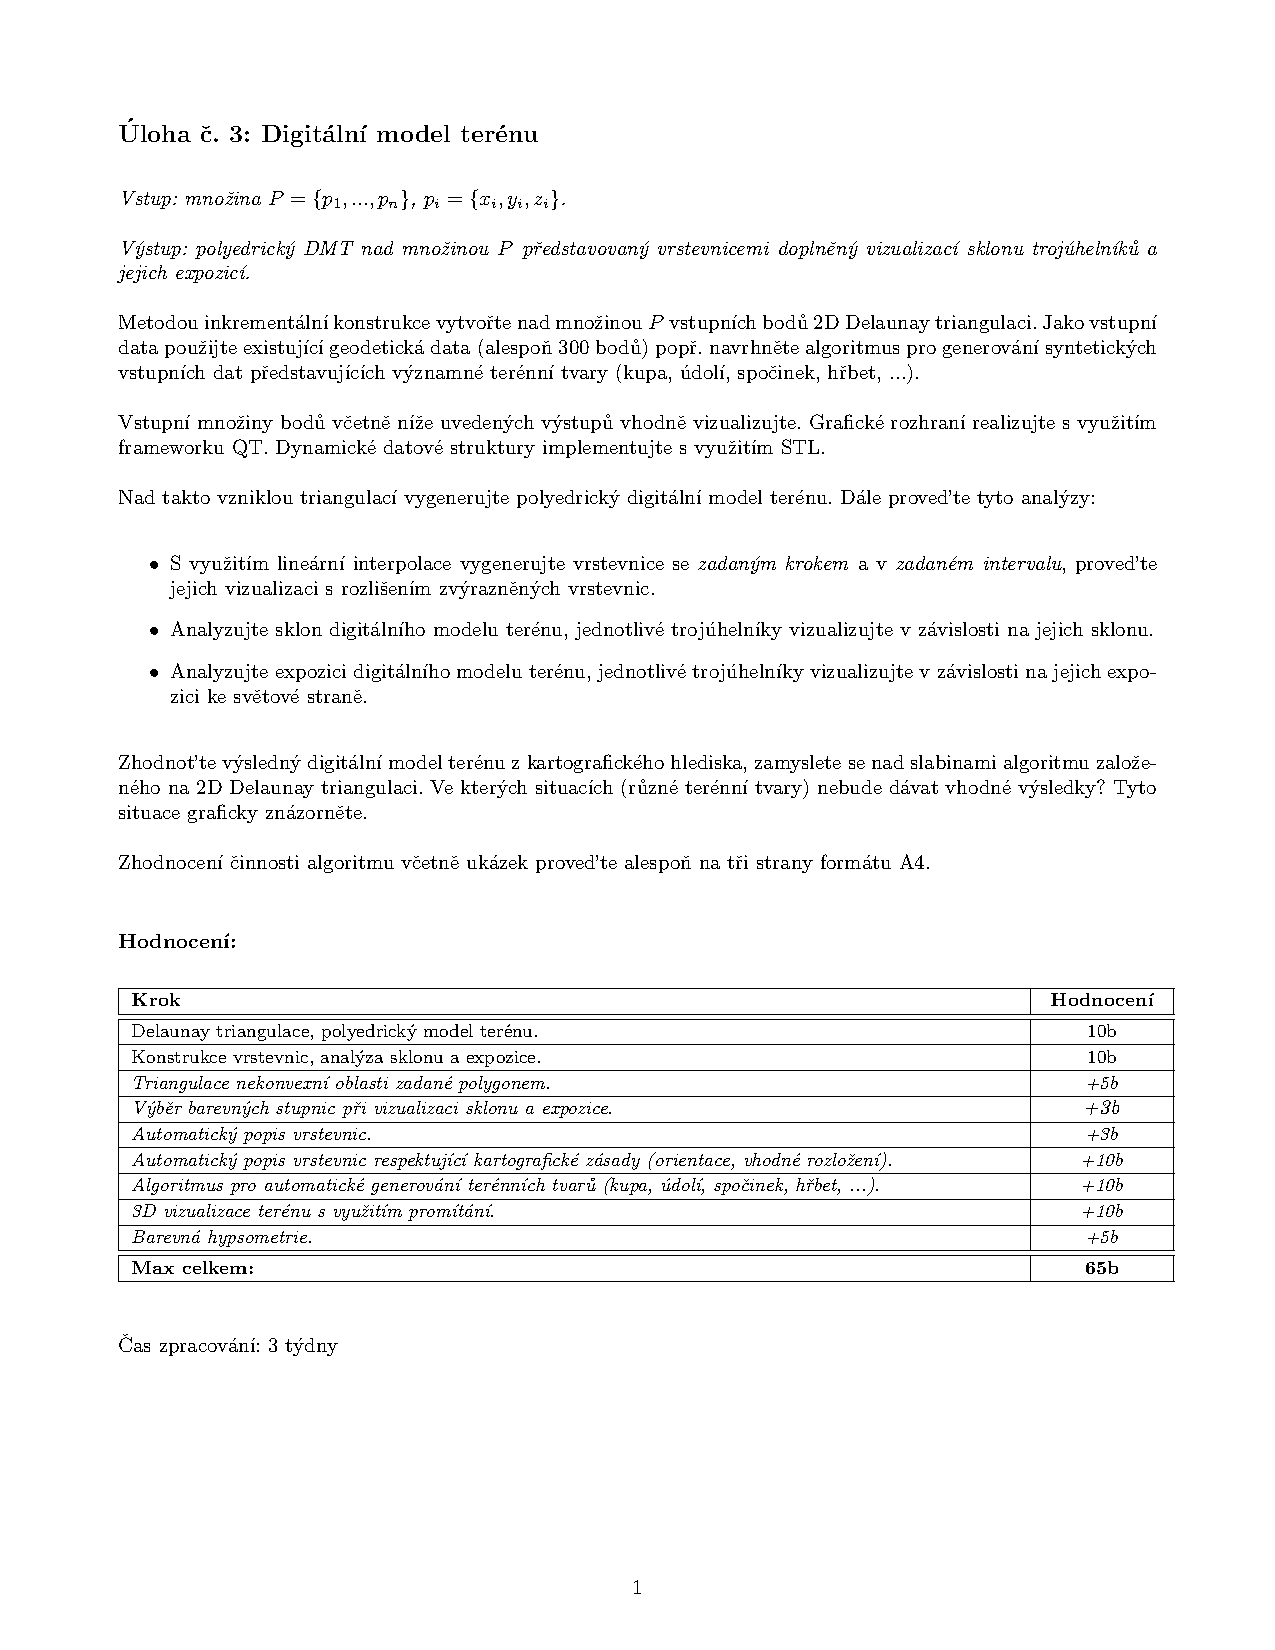
\includegraphics[clip, trim=0cm 5cm 0cm 3cm, width=1.0\textwidth]{zadani.pdf}
\end{figure}


\section{Údaje o bonusových úlohách}




\clearpage

\section{Popis a rozbor problému}

Mějme množinu $P {p_i}$ bodů $p_i = {x_i, y_i, z_i}$. Nad tuto množinou chceme vytvořit síť trojúhelníků $t_j$ pomocí Delaunay triangulace $DT$. 

Vlastnosti Delaunay triangulace:

\begin{itemize}
\item Uvnitř kružnice opsané trojúhelníku $t_j \in DT$ neleží žádný jiný bod množiny P.
\item $DT$ maximalizuje minimální úhel v $\forall t_j$, avšak $DT$ neminimalizuje maximální úhěl v $t_j$

\item $DT$ je lokálně optimální i globálně optimální vůči kritériu minimálního úhlu
\item $DT$ je jednoznačná, pokud žádné čtyři body neleží na kružnici.
\end{itemize}

Z těchto vlastností také plyne, že trojúhelníky jsou tvořeny tak, aby kružnice jim opsaná byla minimální ze všech možných.




%OBRÁZEK
%\begin{figure}[h]
%	\centering
%	\includegraphics[width=10cm]{KO.png}
%	\caption{Konvexní obálka}
%\end{figure}


\clearpage
\section{Popis algoritmů}

\subsection{Delaunayova triangulace}

\vspace{1.5cm}
\subsubsection{Implementace metody}
\begin{enumerate}
\item $ p_1 = rand(P), ||p_2-p_1|| = min $ ....náhodný a nebližší bod
\item Vytvoř hranu $ e = (p_1,p_2) $ 
\item Inicializuj: $p_{min} = arg min_{\forall p_i\in\sigma_L(e)} r'(k_i), k_i = (a, b, p_i), e = (a,b)$
\item Pokud $ \nexists p_{min},$ prohoď orientaci $e \longleftarrow (b,a) $. Jdi na $3)$
\item $e_2 = (p_1,p_{min}), e_3 = (p_{min},p_1) $...zbývající hrany trojúhelníku
\item $AEL \longleftarrow e, AEL \longleftarrow e_2, AEL \longleftarrow e_3 $
\item $DT \longleftarrow e, DT \longleftarrow e_2, DT \longleftarrow e_3 $ 
\item while AEL not empty:
\item \hspace {1cm} $AEL  \longrightarrow e, e = (p_1, p_2) $....vezme první hranu z AEL
\item \hspace {1cm}$ e = (p_2, p_1)$ ...prohodí její orientaci
\item \hspace {1cm} $p_{min} = arg min_{\forall p_i\in\sigma_L(e)} r'(k_i), k_i = (a, b, p_i), e = (a,b) $
\item \hspace {1cm} if $ \exists p_{min}:$
\item \hspace {2cm} $e_2 = (p_1,p_{min}), e_2 = (p_{min},p_1) $...zbývající hrany trojúhelníku
\item \hspace {2cm} $DT \longleftarrow e  $  
\item \hspace {2cm} $ add(e_2,AEL,DT), add(e_3,AEL,DT)$
\end{enumerate}

Dílčí algoritmus Add:
\begin{enumerate}
	\item Vytvoř hranu $e' = (b,a)$
	\item if $(e' \in AEL)$
	\item \hspace {1cm} $ AEL \longrightarrow e'$...Odstraň z AEL
	\item else:
	\item \hspace {1cm} $ AEL \longleftarrow e$ ...Přidej do AEL
	\item $DT\longleftarrow (a,b)$ Přidej do DT
\end{enumerate}


\clearpage

\subsection{Vrstevnice}

\begin{enumerate}
	\item doplnit
\end{enumerate}


\subsubsection{Implementace metody}
\begin{enumerate}
	\item doplnit
\end{enumerate}

\subsection{Sklon}

\subsection{Expozice}


% ===============================================================

\section{Vstupní data}

Vstupními daty je množina bodů, kterou lze zadat dvěma způsoby:\\
1) klikáním na kanvas\\
2) použitím generátoru bodů, který je součástí aplikace, přičemž se body generují dle zadaných kritérií.\\

%--------------------------------------------------------------------------------------------------------------------------------------

\clearpage
\section{Ukázka vytvořené aplikace}


\clearpage


Nejprve je třeba zadat vstupní data - množinu bodů.\\


Následně je možné vybrat metodu výpočtu konvexní obálky a kliknutím na tlačítko GO v 
sekci Create convex hull zahájen výpočet a vizualizace konvexní obálky zadané množiny bodů.
Pod tlačítkem Go je vypsán čas, jak dlouho trval výpočet.\\


Vše je uvedeno do původního stavu (smazány body i vypočtené vyýsledky) kliknutím na tlačítko Clear.\\

\clearpage

%=======================================================================================



\subsection{Algorithms}
V třídě Algorithms jsou staticky implementovány algoritmy počítající kovexní obálku a minimální ohraničující obdélník (včetně vodící linie).

\begin{itemize}

	\item Výčtový typ \textbf{TPosition}
		\begin{itemize}
			\item Typ využitý jako návratová hodnota členské metody \textbf{getPointLinePosition}.
			\item \textbf{LEFT = 0}
			\item \textbf{RIGHT = 1}
			\item \textbf{ON = 2}
		\end{itemize}

	\item Metoda \textbf{getPointLinePosition}
		\begin{itemize}
			\item Tato metoda slouží k určení polohy bodu vůči přímce. Návratovou hodnotou je výčtový typ \textbf{TPosition}.
			\item Vstup
				\begin{itemize}
					\item \textbf{QPointF \&q} - určovaný bod
					\item \textbf{QPointF \&a, \&b} - body přímky
				\end{itemize}
			\item Výstup
				\begin{itemize}
					\item \textbf{LEFT} - bod vlevo od přímky
					\item \textbf{RIGHT} - bod vpravo od přímky
					\item \textbf{ON} - bod na přímce
				\end{itemize}

		\end{itemize}

	\item Metoda \textbf{getTwoVectorsAngle}
		\begin{itemize}
			\item Tato metoda slouží k určení úhlu mezi 2 přímkami. Její návratovou hodnotu je \textbf{double}.
			\item Vstup
				\begin{itemize}
					\item \textbf{QPointF \&p1, \&p2} - body první přímky
					\item \textbf{QPointF \&p3, \&p4} - body druhé přímky
				\end{itemize}
		
			\item Výstup
				\begin{itemize}
					\item Úhel mezi 2 přímkami
				\end{itemize}			
		\end{itemize}

	\item Metoda \textbf{getPointLineDistance}
		\begin{itemize}
			\item Tato metoda slouží k výpočtu vzdálenosti bodu od přímky. Její návratovou hodnotou je \textbf {double} %\begin{double.}
			\item Vstup
				\begin{itemize}
					\item \textbf{QPointF \&q} - určovaný bod
					\item \textbf{QPointF \&a, \&b} - body přímky
				\end{itemize}
			\item Výstup
				\begin{itemize}
					\item Vzdálenost bodu od přímky
				\end{itemize}
		\end{itemize}

	\item Přetížená metoda \textbf{rotateByAngle}
		\begin{itemize}
			\item Tato metoda slouží k rotaci dané množiny o úhel. Jejím návratovým typem je \textbf{void}.
			\item Vstup
				\begin{itemize}
					\item Přetížení 1
						\begin{itemize}
							\item \textbf{std::vector$<$QPointF$>$ \&points} - vektor bodů, jež má být orotován
							\item \textbf{double angle} - úhel, o který má rotace být provedena
 						\end{itemize}
					
					\item Přetížení 2
						\begin{itemize}
							\item \textbf{QPolygonF \&points} - polygon, jež má být orotován
							\item \textbf{double angle} - úhel, o který má rotace být provedena
 						\end{itemize}

					\item Přetížení 3
						\begin{itemize}
							\item \textbf{QLineF \&points} - úsečka, jež má být orotována
							\item \textbf{double angle} - úhel, o který má rotace být provedena
 						\end{itemize}					
				\end{itemize}
			
		\end{itemize}

	\item Metoda \textbf{getDistance}
		\begin{itemize}
			\item Tato metoda slouží k výpočtu vzdálenosti dvou bodů. Jejím výstupním typem je \textbf{double}.
			\item Vstup
				\begin{itemize}
					\item \textbf{QPointF \&a, \&b} - body, mezi kterými je vzdálenost počítána
				\end{itemize}
			\item Výstup
				\begin{itemize}	
					\item Vypočtená vzdálenost
				\end{itemize}
		\end{itemize}

	\item Metoda \textbf{jarvisScanCH}
		\begin{itemize}
			\item Tato metoda slouží k výpočtu konvexní obálky pomocí algoritmu Jarvis Scan. Během výpočtu je ošetřována singularita existence kolineárních bodů v datasetu. Jejím výstupním typem je \textbf{QPolygonF}.
			\item Vstup
				\begin{itemize}
					\item \textbf{std::vector} $<$\textbf{QPointF}$>$ \textbf{points} - vektor bodů, kolem nichž má být vytvořená konvexní obálka.
				\end{itemize}
			\item Výstup
				\begin{itemize}
					\item Polygon obsahující kovexní obálku.
				\end{itemize} 
		\end{itemize}

	\item Metoda \textbf{grahamScanCH}
		\begin{itemize}
			\item Tato metoda slouží k výpočtu konvexní obálky pomocí algoritmu Graham Scan. Jejím výstupním typem je \textbf{QPolygonF}.
			\item Vstup
				\begin{itemize}
					\item \textbf{std::vector} $<$\textbf{QPointF}$>$ \textbf{points} - vektor bodů, kolem nichž má být vytvořená konvexní obálka.
				\end{itemize}
			\item Výstup
				\begin{itemize}
					\item Polygon obsahující kovexní obálku.
				\end{itemize} 
		\end{itemize}

	\item Metoda \textbf{quickHullCH}
		\begin{itemize}
			\item Tato metoda slouží k výpočtu konvexní obálky pomocí algoritmu Quick Hull. Jejím výstupním typem je \textbf{QPolygonF}.
			\item Vstup
				\begin{itemize}
					\item \textbf{std::vector} $<$\textbf{QPointF}$>$ \textbf{points} - vektor bodů, kolem nichž má být vytvořená konvexní obálka.
				\end{itemize}
			\item Výstup
				\begin{itemize}
					\item Polygon obsahující kovexní obálku.
				\end{itemize} 
		\end{itemize}

	\item Metoda \textbf{quickHullLocal}
		\begin{itemize}
			\item Pomocná metoda k výpočtu konvexní obálky metodou Quick Hull. Jejím výstupním typem je \textbf{void}.
			\item Vstup
				\begin{itemize}
					\item \textbf{int s, e} - index počátečního a koncového bodu dělící přímky
					\item \textbf{std::vector} $<$\textbf{QPointF}$>$ \&\textbf{points} - vektor bodů, kolem nichž má být vytvořená konvexní obálka.
					\item \textbf{QPolygonF \&poly\_ch} - polygon obsahující body konvexní obálky
				\end{itemize}
			\item Výstup
				\begin{itemize}
					\item Polygon obsahující kovexní obálku.
				\end{itemize} 
		\end{itemize}

	\item Metoda \textbf{sweepLineCH}
		\begin{itemize}
			\item Tato metoda slouží k výpočtu konvexní obálky pomocí algoritmu Sweep Line. Jejím výstupním typem je \textbf{QPolygonF}.
			\item Vstup
				\begin{itemize}
					\item \textbf{std::vector} $<$\textbf{QPointF}$>$ \textbf{points} - vektor bodů, kolem nichž má být vytvořená konvexní obálka.
				\end{itemize}
			\item Výstup
				\begin{itemize}
					\item Polygon obsahující kovexní obálku.
				\end{itemize} 
		\end{itemize}

	\item Metoda \textbf{generatePoints}
		\begin{itemize}
			\item Metoda pro generování zadaného počtu a tvaru bodů. Jejím výstupním typem je \textbf{std::vector} $<$\textbf{QPointF}$>$ \textbf{points}.
			\item Vstup
				\begin{itemize}
					\item \textbf{QSizeF \&canvas\_size} - rozměry kreslícího plátna, ze kterých se determinuje rozsah generovaných bodů
					\item \textbf{int point\_count} - počet bodů, který se má generovat
					\item \textbf{std::string shape} - tvar vytvářené množiny bodů (random, grid, na kružnici, na elipse, na čtverci)
				\end{itemize}
			\item Výstup
				\begin{itemize}
					\item Vektor nagenerovaných bodů.
				\end{itemize}
		\end{itemize}

	\item Metoda \textbf{minimalRectangle}
		\begin{itemize}
			\item Metoda pro výpočet minimálního ohraničujícího obdélníku a hlavní linie. Jejím výstupním typem je \textbf{void}.
			\item Vstup
				\begin{itemize}
					\item \textbf{QPolygonF \&poly\_ch} - polygon obsahující konvexní obálku
					\item \textbf{QPolygonF \&minimal\_rectangle} - polygon, do kterého jsou počítány body minimálního ohraničujícího obdélníku
					\item \textbf{QLineF \&direction} - hlavní linie minimálního ohraničujícího obdelníku (resp. do této proměnné je počítaná)
					\item \textbf{bool compute\_dir\_line} - ukazatel určující zda-li má být počítána hlavní linie minimálního ohraničujícího obdélníku
				\end{itemize}

		\end{itemize}
\end{itemize}
\clearpage

\subsection{Draw}
Třída draw slouží k vykreslení vygenerovaných (nebo naklikaných) bodů, vypočteného minimálního ohraničujícího obdélníku a hlavní linie minimálního ohraničujícího obdélníku. V této třídě jsou zároveň nagenerované body zbavené duplicit a vypočtené konvexní obálky se zde omezují na striktní konvexní obálky (vše v metodě \textbf{setCH}. Třída dědí od třídy \textbf{QWidget}. 

\begin{itemize}
	\item Členské proměnné
		\begin{itemize}
			\item \textbf{std::vector} $<$\textbf{QPointF}$>$ \textbf{points} - vektor obsahující nagenerované nebo naklikané body
			\item \textbf{QPOlygonF ch} - polygon obsahující body konvexní obálky
			\item \textbf{QPolygonF rect} - polygon obsahující body minimálního ohraničujícího obdélníku
			\item \textbf{QLineF direction} - hlavní linie minimálního ohraničujícího obdélníka
		\end{itemize}

	\item Metoda \textbf{paintEvent}
		\begin{itemize}
			\item Tato metoda slouží k vykreslení nagenerovaných (nebo naklikaných) bodů, konvexní obýlky, minimálního ohraničujícího obdélníka a hlavní linie minimálního ohraničujícího obdélníka. Metoda se volá pomocí metody \textbf{repaint()}. Návratovým typem je \textbf{void}.
			\item Vstup
				\begin{itemize}
					\item \textbf{QPaintEvent *e}
				\end{itemize}
		\end{itemize}

	\item Metoda \textbf{mousePressEvent}
		\begin{itemize}
			\item Metoda sloužící k uložení bodu do členské proměnné \textbf{points} určeného kliknutím myší nad kreslícím plátnem. Jejím návratovým typem je \textbf{void}.	
			\item Vstup
				\begin{itemize}
					\item \textbf{QMouseEvent *e}
				\end{itemize}
		\end{itemize}

	\item Metoda \textbf{setCH}
		\begin{itemize}
			\item Tato metoda slouží pro kontrolu duplicity generovaných bodů, pro kontrolu alespoň 3 bodů, k zavolání příslušného algoritmu pro vypočtení konvexní obálky a k omezení konvexní obálky na striktně konvexní obálku. Metoda počítá dobu trvání výpočetních algoritmů. Jejím návratovým typem je \textbf{double}.
			\item Vstup
				\begin{itemize}
					\item \textbf{std::string \&selected\_algorithm} - uživatelsky vybraný algoritmus pro počítání konvexní obálky
				\end{itemize}
			\item Výstup
				\begin{itemize}
					\item Čas trvání výpočtu.
				\end{itemize}
		\end{itemize}	

	\item Metoda \textbf{setRect}
		\begin{itemize}
			\item Tato metoda slouží pro zavolání algoritmu pro výpočte minimálního ohraničujícího obdélníku a jeho hlavní linie. Jejím návratovým typem je \textbf{void}.
			\item Vstup
				\begin{itemize}
					\item \textbf{bool draw\_dir\_line} - uživatelsky nastavený indikátor, zda-li se má vypočítat hlavní linie minimálního ohraničujícího obdélníku
				\end{itemize}
		\end{itemize}

	\item Metoda \textbf{setPoints}
		\begin{itemize}
			\item Metoda volající algoritmus pro generování bodů daného počtu a tvaru. Jejím návratovým typem je \textbf{void}.
			\item Vstup
				\begin{itemize}
					\item \textbf{QSizeF \&canvas\_size} - rozměr kreslícího plátna pro pozdější určení rozsahu generování bodů
					\item \textbf{int count} - počet bodů, jež se má generovat
					\item \textbf{std::string \&shape} - tvar, do kterého se body mají generovat
				\end{itemize}
		\end{itemize}

	\item Metoda \textbf{clearCanvas}
		\begin{itemize}
			\item Metoda, která maže obsah kreslícího okna. Jejím návratovým typem je \textbf{void}. Do metody nevstupují žádné parametry.
		\end{itemize}
\end{itemize}

\subsection{SortByXAsc, SortByYAsc, SortByAngleAsc}
Třídy sloužící jako sortovací kritérium - podle rostoucí souřadnice x resp. souřadnice y (při stejných souřadnicích x resp. y je druhým kritériem druhá souřadnice) a podle rostoucího úhlu mezi body (při stejném úhlu je druhým kritériem vzdálenosti mezi body).
\clearpage

\subsection{Widget}
Tato třída slouží ke komunikaci s GUI. Třída dědí od třídy QWidget. Všechny její metody slouží jako sloty k signálům z GUI, nemají žádné vstupní hodnoty a jejich návratovým typem je void. 

\begin{itemize}
	\item Metoda \textbf{on\_createCHButton\_clicked} - reaguje na zmáčknutí tlačítka pro vypočtení konvexní obálky, volá metodu \textbf{setCH} z třídy \textbf{Draw}, zapisuje čas výpočtu do GUI.

	\item Metoda \textbf{on\_generateButton\_clicked} - reaguje na zmáčknutí tlačítka pro generování bodů, volá metodu \textbf{setPoints} z třídy \textbf{Draw}.

	\item Metoda \textbf{on\_clearButton\_clicked} - reaguje na zmáčknutí tlačítka pro vymazání obsahu kreslícího plátna, volá metodu \textbf{clearCanvas} z třídy \textbf{Draw}.

	\item Metoda \textbf{on\_createRectButton\_clicked} - reaguje na zmáčknutí tlačítka pro vypočtení minimálního ohraničujícího obdélníka, volá metodu \textbf{setRect} z třídy \textbf{Draw}.

	\item Metoda \textbf{on\_helpButton\_clicked} - reaguje na zmáčknutí tlačítka pro volání nápovědy, volá okno s nápovědou \textbf{help\_dialog} z třídy \textbf{HelpDialog}.

\end{itemize} 

\vspace{3cm}
\subsection{HelpDialog}
Třída sloužící pro vykreslení okna s nápovědou.

\clearpage

\section{Přílohy}

\begin{itemize}
	\item Príloha č.1: Testování výpočetních dob algoritmů - "Testovani.pdf"
\end{itemize}
 %--------------------------------------------------------------------------------------------------------------------------------------------------------------------------
\clearpage
\section{Závěr}

\subsection{Politování se a vysvětlení našeho problému}
Aplikace od začátku implementovala body, polygony, linie atd. v typu float (QPointF, QPolygonF, QLineF), v tomto duchu byly psány i všechny algoritmy. Při testování bylo zjištěno, že výpočet takto implementovaných algoritmů trvá VELMI dlouho (v řádu stovek sekund). Proto bylo navrženo (dva dny před odevzdáním), že by bylo vhodné vyzkoušet, jak budou algoritmy rychle počítat při implementaci bodů, polygonů a linií v typu int (QPoint, QPolygon, QLine). Bylo zjištěno, že tato změna (aplikovaná pomocí programu grep (to jsme se jen chtěli pochlubit, že jsme to zmákli přepsat rychle)) algoritmy rapidně urychlí (do řádu sekund až sub-sekund). Z tohoto důvodu (a také z časových důvodů, při testování pomalejší verze počítač zamrzá a člověk u toho musí pořád sedět a odklikávat "Wait", aby program nepadl) jsou uvedeny grafy z testování rychlejší verze. Kdyby všechny algoritmy po tomto přechodu fungovaly správně, ani bychom se neobtěžovali psát tak obsáhlý závěr, ale to by nebyla smůla, aby se to nerozbilo. Především myšlenka rotací tam a zpět u minimálního ohraničujícího obdélníku již nefunguje - orotované souřadnice se zaokrouhlí na celé číslo, při rotaci zpět se opět zaokrouhlí na celé číslo a problém je na světě. \\
Dále je jakýmsi neidentifikovatelným způsobem rozbitý výpočet Jarvis Scan na kružnici (kód jsme změnili na kód stejný jako z hodiny, kód generování bodů na kružnici máme obdobný jako ostatní skupinky, ale i tak nefunguje úplně správně, neumíme určit problém (a moc nás to mrzí (skutečně, neironicky (to taky není ironie)))). Jelikož jsme strávili spoustu hodin nad co nejoptimálnější implementací těchto algoritmů a samozřejmě jsme to celou dobu testovali pro malé množiny bodů, kdy vše běží rychle, rozhodli jsme se odevzdat 2 verze kódu. Složky jsou pojmenované \texttt{src\_float} pro původní super vymazlenou verzi a \texttt{src\_int} pro testovací rozbitou verzi s tím, že si stojíme za super vymazlenou verzí \texttt{src\_float}, kde funguje vše, ale pro velké množství bodů v některých případech pomaleji (hlavně Jarvis Scan). Jako release odevzdáváme verzi \texttt{src\_float}. Doufáme, že to takto bude v pořádku.\\
 Ještě bychom se rádi pochlubili šikovnou implementací vymazávání duplicitních bodů při generování množin (nejprve jsme sortovali, a pak porovnávali následující body, uložili vždy poslední stejný, takto nemusíme použít vnořený cyklus a náročnost je lineární a ne kvadratická).

\subsection{Návrhy na vylepšení}
\begin{itemize}
	\item Přizpůsobení vykreslených prvků při zvětšování/zmenšování okna
	\item Úplné vynechání Jarvis Scanu
	\item Lepší algoritmus na počítání minimálního ohraničujícího obdélníka, nejlépe takový, při kterém se nemusí rotovat celá množina bodů
		\begin{itemize}
			\item Krom šikovných algoritmů z prezentace by také šla využít analytická geometrie, tj. v podstatě stejný postup jaký jsme použili v našem programu, ale nerotovalo by se:
				\begin{itemize}
					\item V cyklu by se opět procházely všechny strany, ty by byly proloženy vždy přímkou p. 
					\item Přímce p by se našel nejvzdálenější bod, vedla by se jím přímka q $||$ p a přímka k kolmá na p a q.
					\item Přímce k by se našel nejvzdálenější bod vlevo, jím by se vedla přímka kl kolmá na p a q.
					\item Přímce k by se našel nejvdálenější bod vpravo, jím by se vedla přímka kp kolmá na p a q.
					\item Našly by se průsečíky přímek p a kl, p a kp, q a kl, q a kp jako souřadnice rohů ohraničujícího obdélníku.
					\item Dále by byl postup totožný s postupem v našem programu (testování velikosti obsahu ohraničujícího obdélníku).
				\end{itemize}
		\end{itemize}
	\item Optimalizace velikosti vykreslovaných značek bodů vzhledem k počtu vykreslených bodů (tak aby byla lépe vidět konvexní obálka).
\end{itemize}

\clearpage
\section{Zdroje}

\begin{enumerate}
\item  BAYER, Tomáš. Konvexní obálky [online][cit. 21.10.2018]. \\
Dostupné z: https://web.natur.cuni.cz/~bayertom/images/courses/Adk/adk4.pdf  \\

\item  BAYER, Tomáš. Konvexní obálky [online][cit. 30.11.2018]. \\
Dostupné z: https://web.natur.cuni.cz/~bayertom/images/courses/Adk/adkcv2.pdf\\
%=======================================================================================
\end{enumerate}
\end{document}



 
